\section{Analysis}

\subsection{Exploratory Data Analysis}
Before building our model, we first wanted to understand the data that we were building our model on. Below is the summary statistics for quantitative variables.

\subsection{Quantitative variables}
Summary Statistics of Quantitative Variables
Min, 1st Quartile, Median, Mean, 3rd Quartile, Max of quantitative variables
\input{quantitative_summary, file = '../../data/eda.txt'}
Range of Quantitative Variables
\input{quantitative_range, file = '../../data/eda.txt'}
IQR of Quantitative Variables
\input{quantitative_IQR, file = '../../data/eda.txt'}
Standard Deviation of Quantitative Variables
\input{quantitative_SD, file = '../../data/eda.txt'}

These histograms will help us better understand the distributions of some of the more relevant quantitative variables.

\subsection{Histogram}
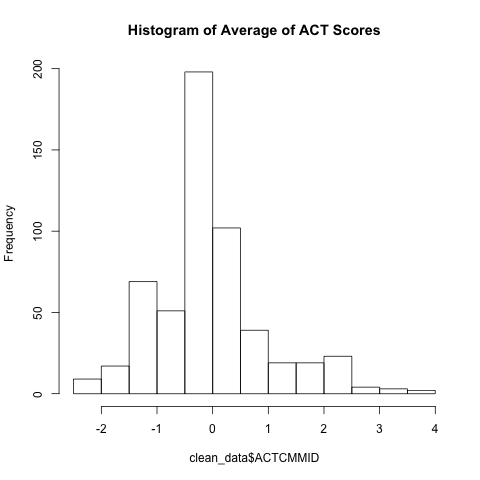
\includegraphics{../../images/histogram_ACT_avg.png}
The total score of the ACT is 36.
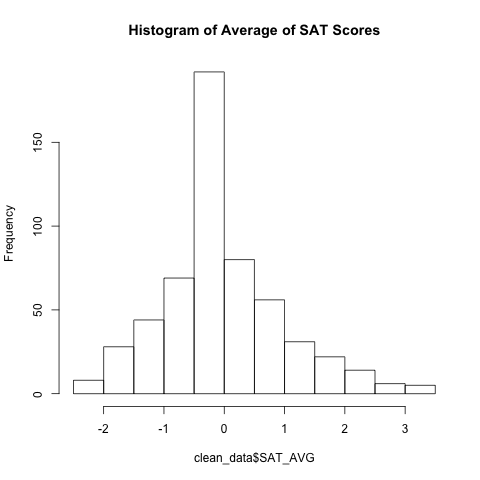
\includegraphics{../../images/histogram_SAT_avg.png}
The total score of the SAT is 2400.
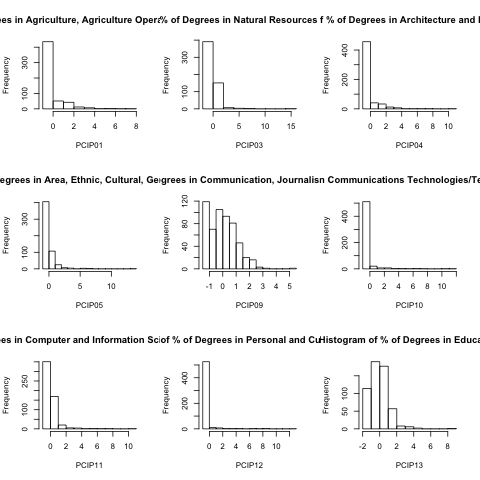
\includegraphics{../../images/histogram_majors1.png}
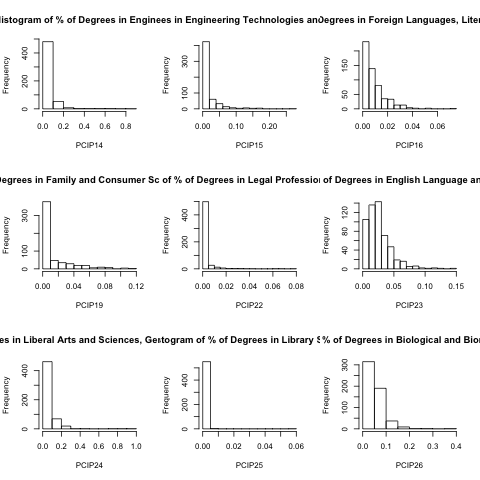
\includegraphics{../../images/histogram_majors2.png}
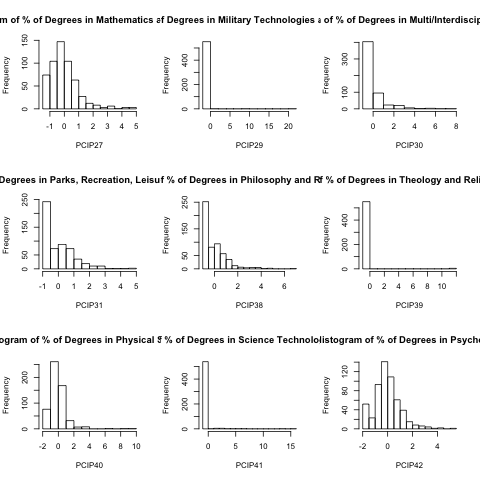
\includegraphics{../../images/histogram_majors3.png}
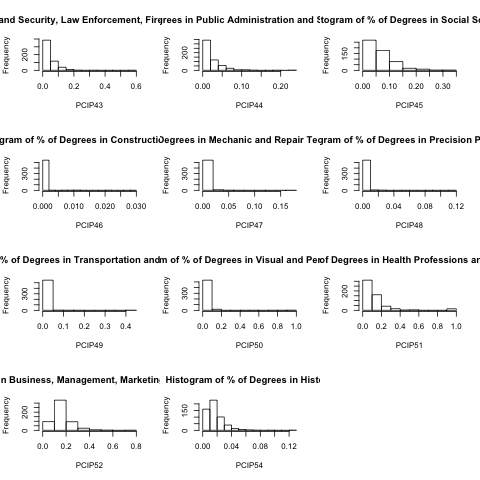
\includegraphics{../../images/histogram_majors4.png}
The following histograms shows us the percentage of degrees in each respective major. We can see that ... major has a lot more percentage than ... major.
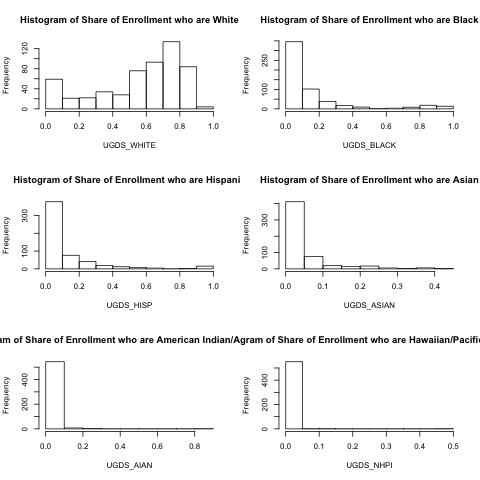
\includegraphics{../../images/histogram_race_enrollment.png}
Comparing the histograms of enrollment by race, ... has the most enrollment and ... has the least enrollment.
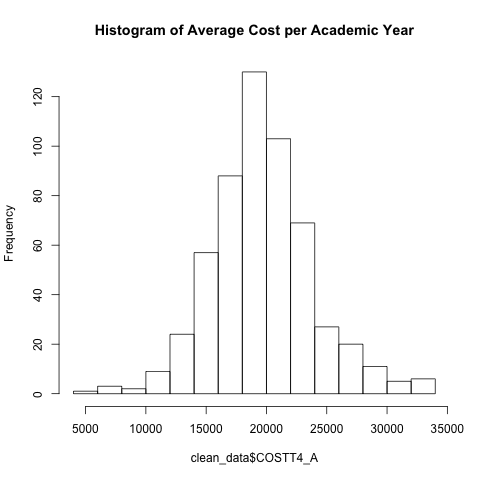
\includegraphics{../../images/histogram_net_price.png}
This histogram shows us the average net price of enrollment.
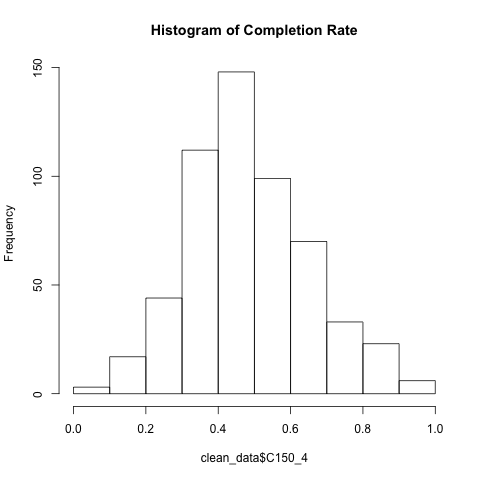
\includegraphics{../../images/histogram_completion.png}
This histogram shows us the average completion rate in 6 years.
\includegraphics{../../images/histogram_income_graduation.png}
Comparing the histograms of completion rate by income, students from ...-income families have the highest completion rate and students from ...-income families have the lowest completion rate.
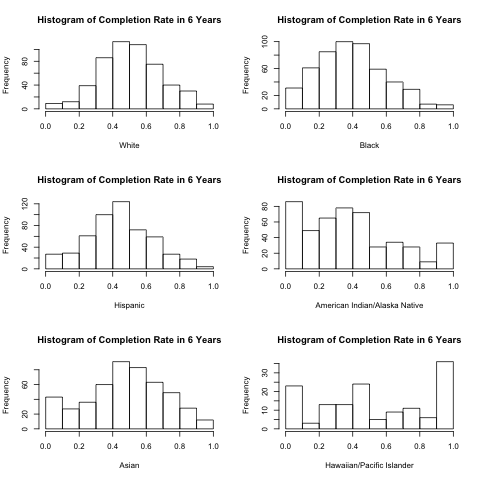
\includegraphics{../../images/histogram_race_completion}
Last but not least, comparing the histograms of completion rate by race, ... students have the highest completion rate and ... students have the lowest completion rate.

From the above histograms, we can have a general idea of the distribution and maybe which variables affects graduation rate. However, to have a more concrete idea, we want to do further analysis.

\subsection{Qualitative variables}
Summary Statistics of Qualitative Variable
\input{summary_qual, file = '../../data/eda.txt'}
Table of Frequency of qualitative variable
\input{freq_qual, file = '../../data/eda.txt'}

\subsection{Exploratory Graphics (qualitative variables)}
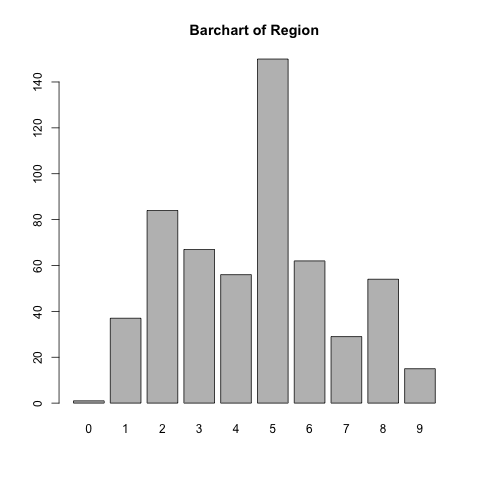
\includegraphics{../../images/barchart_region.png}
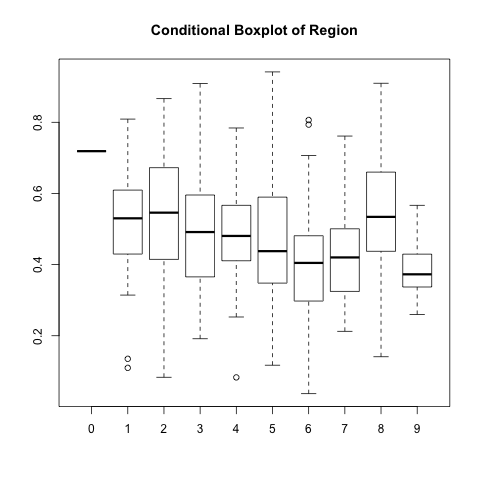
\includegraphics{../../images/conditional_boxplot_region.png}

### SHOW LASSO AND BIC PLOTS
